In this chapter we present the basic theory behind Large Language Models. We then introduce the LLaMA family of models, which we've been using. Subsequently, we describe the embedding technique we've used and we present our results.

\section{Vocabulary}

The following vocabulary is used:
\begin{itemize}
	\item \textbf{Token} is a basic unit of text data a language model processes - usually words, subwords, punctuation marks etc.

	\item \textbf{Tokenization} is a process of breaking down input data into tokens.

	\item \textbf{Language model} is a \textit{probabilistic model} of a natural language. Probabilistic - meaning that given some input text data, it's job is to predict the future token. \cite{language_models}

	\item \textbf{Supervised learning} is a type of a method of training machine learning models where every input is supplied with the output the model is expected to produce. The model then matches its own output with the expected output to correct its own behaviour.

	\item \textbf{Pretraining} is a process of training the language model on a corpus of data

	\item \textbf{Fine-tuning} is a process of adapting a pretrained language model to a specific task (e.g. mathematics, poetry) by training it on a smaller, task-specific dataset.

	\item \textbf{Token embedding} is a mapping of tokens to high-dimensional vectors of real numbers. This mapping is expected to have the property that tokens similar in meaning are close in the output space. See \cite{token_embeddings}.

	\item \textbf{Context length} is the maximal size of input tokens a large language model can process at any one time.

	\item \textbf{Cross-modality data} is data that combines multiple modalities, i.e. text, image, audio, video, etc. In particuliar, combination of text description and time series is cross-modality data.

\end{itemize}
% CLEAN

\section{Overview}

A Large Language Model (LLM) \cite{llmintro} is a language model that is pretrained on a large collection of data (usually billions of tokens).
%an advanced artificial intelligence system designed to understand and generate human-like text based on patterns it learns from enormous amounts of textual data.
These models utilize deep learning techniques, particularly neural networks, which consist of interconnected neuron layers that process information sequentially, one by one.
The predominant architecture underpinning most contemporary LLMs is the Transformer (see below), notable for its self-attention mechanism that enables the model to assess the importance of different tokens in a sentence irrespective of the order the tokens are in.

The training of an LLM involves pretraining it with a large, diverse corpus of text, during which it adjusts its internal parameters to minimize the difference between its predictions and the actual data. This process of supervised learning equips the model with a probabilistic understanding of the language (its patterns, semantics, syntax, knowledge of the world inherent in a language), enabling it to predict a continuation of a given piece of input text.

Once trained, LLMs can perform a variety of language-based tasks such as translation, summarization, question answering, and text generation.
It can then be fine-tuned to perform better on a specific task, e.g. write poetry, give cooking advice, write programming code, etc.
%Their capability to generate coherent and contextually relevant text makes them invaluable for applications in natural language processing (NLP), including conversational agents, content creation tools, and sophisticated text analysis. 
We will see how such a model deals with analysing and predicting time series data.


\section{The Transformer}

The Transformer is a type of neural network architecture introduced in the seminal 2017 paper \textit{"Attention is All You Need"} by Vaswani et al. \cite{attention_is_all_you_need}. It has since become foundational for many natural language processing (NLP) models due to its efficiency and effectiveness in handling data sequences, such as text.

\subsection{Components}

\begin{figure}[h!]
	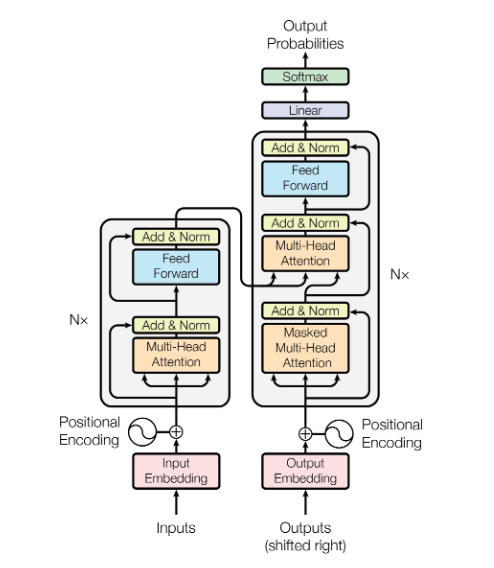
\includegraphics[width=\linewidth]{"pictures/the-transformer-model-architecture.png"} % TODO: better diagram
	\caption{The Transformer model architecture (figure from \cite{attention_is_all_you_need}). Both inputs and outputs are embedded and concatinated (\(\oplus\)) with their positional encodings - those are then fed into encoder and decoder respectivaly. The left part is one encoder layer. The whole encoder is made up of \(N\) of these layers stacked (output of one is input of the next). The output of the last encoder layer is used in all \(N\) decoder layers (on the right), which are likewise stacked. The output of the decoder (stack of decoder layers) is used for prediction.}

	\label{fig:transformer_architecture_fig}
\end{figure}

The Transformer (fig \autoref{fig:transformer_architecture_fig}) consists of the following components:

\begin{enumerate}
	\item \textbf{Input Embedding}: Converts input tokens into vectors.
	\item \textbf{Positional Encoding}: Adds positional information to the embeddings to retain the order of the sequence. This encoding is another high-dimensional vector.
	\item \textbf{Encoder} (\autoref{fig:transformer_architecture_fig} the left):
	      \begin{itemize}
		      \item Consists of \(N = 6\) layers\footnote{\cite{attention_is_all_you_need}, section 3.1}.
		      \item Each layer has two sub-layers:
		            \begin{itemize}
			            \item \textbf{Multi-Head Attention}: Applies attention mechanism over the input. For each token calculates the weight or importance of over tokens in the surrounding context (\textit{Attention}). Does so independently with \(h\) 'heads'\footnote{In \cite{attention_is_all_you_need}, \(h = 6\)}, each calculating different semantic relantionships (\textit{Multi-Head}). The results are concatenated and linearly transformed into size of one output (as if from one head).
			            \item \textbf{Feed Forward}: Applies a fully connected feed-forward neural network.
		            \end{itemize}
		      \item \textbf{Add \& Norm}: Residual connections followed by layer normalization after each sub-layer.
	      \end{itemize}
	\item \textbf{Decoder} (\autoref{fig:transformer_architecture_fig}, on the right):
	      \begin{itemize}
		      \item Also consists of \(N = 6\) layers\footnote{\cite{attention_is_all_you_need}, section 3.1}.
		      \item Each layer has three sub-layers:
		            \begin{itemize}
			            \item \textbf{Masked Multi-Head Attention}: As in Encoder, but masked, i.e. attention results for future tokens are disarded - .
			            \item \textbf{Multi-Head Attention}: Applies the multi-head attention mechanism to encoder output.
			            \item \textbf{Feed Forward}: Applies a fully connected feed-forward neural network.
		            \end{itemize}
		      \item \textbf{Add \& Norm}: Residual connections followed by layer normalization after each sub-layer.
	      \end{itemize}
	\item \textbf{Output Embedding}: Converts decoder output tokens into semantic vector space.
	\item \textbf{Linear \& Softmax Layer}: Maps the decoder’s output to the probability distribution over the target vocabulary. The most probable token is the output. \footnote{This may seem contrary to popular experience using e.g. ChatGPT, where given the same input, it may not necessarily output the same result. However, such tools may have random seeds for each interaction session and also may take into account the context of the conversation. }
\end{enumerate}




\section{LLaMA model}

\subsection{Introduction}
\textbf{LLaMA} or \textit{Large Language Model Meta AI} \cite{llama} is a collection of large language models developed by Meta AI.

\subsection{Features}

\begin{itemize}
	\item \textbf{Model Variants:} LLaMA is available in various sizes, offering flexibility for deployment in different environments. These variants range from models of 7 billion parameters in size up to models of 65 billion parameters in size. \footnote{LLaMa-3, which came out in April 2024, has size possibilities of 8 billion and 70 billion parameters}

	\item \textbf{Training Data:} The model has been trained on 1.4 trillion tokens of data from several sources, including CommonCrawl and Github, Wikipedia (Table 1. in \cite{llama}). It therefore has an enormous and domain diverse range of input data.

	      % \item \textbf{Application Scope:} Due to the possibility of using different sizes, LLaMA is suited for a variety of applications, such as conversational agents, content generation, summarization, and more advanced tasks like sentiment analysis and machine translation.

	\item \textbf{Accessibility:} The code that can be used to run the model has been publicly released under the open-source GPLv3 license \cite{llama_code}.
\end{itemize}

\subsection{LLaMA-2}
\textbf{LLaMA-2} \cite{llama2} is an improved version of LLaMA, with similar model sizes. It has the same architecture as LLaMA-1, but was trained on a much larger set of data (~2 trillion tokens). It also has doubled context length of 4096 tokens. For our experiments, we were using LLaMA-2.

\section{Time-series Embedding}
We now present the technique we've used for using a vanilla (not fine-tuned) LLaMA-2 model to predict time series data.
The main idea involves using a framework around a frozen LLM (i.e. one that is not changed during the training process) that transforms input time series data into a text representation the LLM can then work on. Its output is then converted into a prediction. The idea is due to an article by Jin et al. (2024) \cite{reprogramming_llm}.

\begin{figure}[h!]
	\centering
	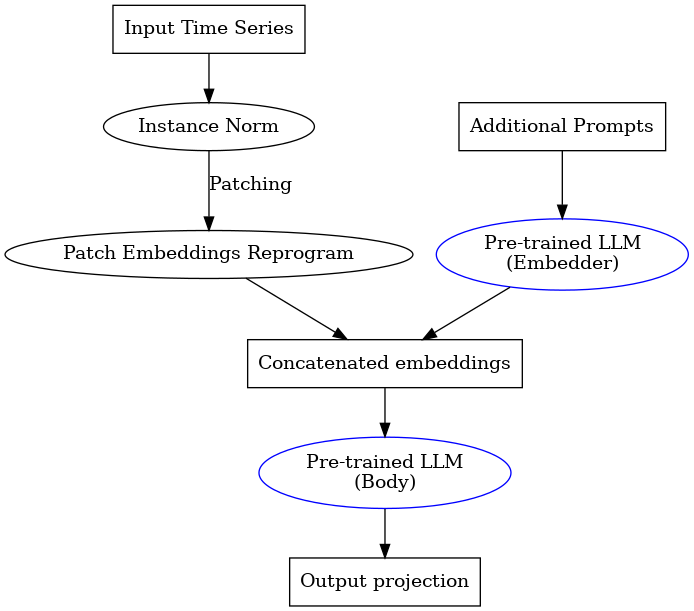
\includegraphics[width=0.5\linewidth]{"pictures/graph.png"}
	\caption{Simplified model of the embedding framework.
		The input time series is normalized and patched (broken down into chunks). These patches are reprogrammed into embeddings,
		and concatenated with embeddings generated from additional prompts by a pre-trained LLM.
		The combined embeddings are then processed by the LLM to produce the final forecast output. }

	% An input time series is normalized, tokenized and embedded,
	% then concatinated together with embedded text prompts. This serves as input to the frozen LLM, which outputs the prediction.}
	% \caption{Simplified model of the embedding framework. Given an input time series, we first tokenize and
	% 	embed it via (1) patching along with a (2) customized embedding layer. (3) These patch embeddings
	% 	are then reprogrammed with condensed text prototypes to align two modalities. To augment the
	% 	LLM’s reasoning ability, (4) additional prompt prefixes are added to the input to direct the transformation
	% 	of input patches. (5) The output patches from the LLM are projected to generate the forecasts.}
	\label{fig:prompt_embedding_fig}
\end{figure}



The following three paragraphs come from the article.\cite{reprogramming_llm}

% TODO: This paragraph/problem may also be described earlier, e.g. in introduction.
\textit{We consider the following problem: given a sequence of historical observations \(X \in \R^{N\times T}\)
	consisting of \(N\) different 1-dimensional variables across \(T\) time steps, we aim to reprogram a large
	language model \(f(\cdot)\) to understand the input time series and accurately forecast the readings at \(H\) future time steps, denoted by \(\hat{Y} \in \R^{N\times H}\) , with the overall objective to minimize the mean square errors between the expected outputs \(Y\) and predictions, i.e., \(\frac1H \sum_{h=1}^H \| \hat{Y}_h - Y_h \|_F^2 \).}

% TODO: normalization, patching, embedding - explain
\textit{The method encompasses three main components: (1) input transformation, (2) a pre-trained and frozen LLM, and (3) output projection. Initially, a multifeature time series is partitioned into \(N\) unifeature time series, which are subsequently processed independently (Nie et al., 2023) \cite{nie_et_al}.
	The i-th series is denoted as \(X(i) \in \R^{1\times T}\) , which undergoes normalization, patching, and embedding prior to being reprogrammed with learned text prototypes to align the source and target modalities.
	Then, we augment the LLM’s time series reasoning ability by prompting it together with the transformed series to generate output representations, which are projected to the final forecasts \(\hat{Y}^{(i)} \in \R^{1\times H}\) .}

\textit{We note that only the parameters of the lightweight input transformation and output projection are updated, while the backbone language model is frozen.
	In contrast to vision-language and other multimodal language models, which usually fine-tune with paired cross-modality data, this use of model is directly optimized and becomes readily available with only a small set of time series and a few  training epochs, maintaining high efficiency and imposing fewer resource constraints compared to building large domain-specific models from scratch or fine-tuning them.}

\section{Our methodology}
In the current and the next few sections we will share the details of our implementation. The goal is to further elaborate on the idea presented in the previous section and describe the specifics and challenges of our approach. \\

Our model has the same architecture as the one presented in the one described in the previous section. We will expand on each of the main components of the model and explain how it is trained.

\subsection{Input Transformation}

\subsubsection*{Data Preprocessing}
As it was previously mentioned, the input to the model is a vector of floating-point numbers representing prices over time. Consequently, we use only use the target feature from the time series data. This implies that, from the datasets described earlier, all columns except the target column are discarded. Following this, the data is normalized.

Each entry in the updated dataset comprises two features. The first feature is a vector of length \textbf{seq\_len} consisting of consecutive prices sampled at intervals of \textbf{seq\_step} values from the original dataset. The second feature is the target feature, which represents the next \textbf{pred\_len} prices, also sampled using the same step size.

\subsubsection*{Embedding}
The embedding in LLaMa2 involves transforming human language into a format that the model can understand and process. The process converts text into a sequence of tokens and later vectors, which are essentially numerical representations of words. First, the text is tokenized. Each token is then mapped to a corresponding vector of floating-point numbers, creating the embedding. The embedding is supposed to capture semantic information about the tokens, allowing the model to understand the meaning of a word in a specific context.

We use predefined methods to perform the embedding in order to provide the model with instructions and additional information about the nature of the dataset and the upcoming input. The details about the prompt will be described in a separate section. The embedded prompt is later used as a part of the input to the model.

\subsubsection*{Patching}
Patches are small, contiguous segments of the original data sequence, representing local windows of information. By patching we mean a preprocessing of the input feature that is meant to prepare it for the model. It is composed of 2 main steps, which are Patch Embedding and Reprogramming. Considering that the weights of the LLM are frozen, patching plays a crucial role in training the model.

\paragraph{Patch Embedding}
The method is used to transform raw input data into a format suitable for sequence modeling. It begins by padding the input through repetition to ensure that patches can be extracted without losing boundary information. Afterwards, we divide the input into overlapping patches, each capturing a segment of the sequence. The patches are then projected into a lower-dimensional space using a 1D convolutional layer, which captures local patterns within a single patch. This provides additional information about the data. Additionally, dropout is applied to the embedded patches in order to prevent overfitting. The resulting sequence, now embedded and regularized, is used as the input for subsequent layers in the model.

\paragraph{Reprogramming}
The purpose of this step is to enchance the LLM's ability to understand the input data. At the moment the input may be seen as random to the model, so in this step we combine the input vector and the instructions embeddings mentioned in the previous section. A linear transformation with unforzen weights is applied to both. Then, multi-head attention is applied to the input using the instructions embeddings.

Finally, the reprogrammed embeddings are reshaped and passed through the output projection layer, which transforms them back into the appropriate dimensionality for the model's subsequent layers. This allows the LLM to understand the connection between the instructions and the input vector.

\subsection{Body and Output Projection}
Two sequences of vectors received from the patching and embedding layers are concatenated and fed into the LLaMa as a single sequence. The output is then projected to the forecasted values using a linear layer.


\subsection{Training Process}

TODO

\section{Model Parameters}
In this study, we employed a set of distinctive parameters for our model training:

\begin{itemize}
	\item \textbf{seq\_len} – This parameter defines the number of records in one prompt to the model.
	\item \textbf{pred\_len} – This parameter specifies the number of records to predict.
	\item \textbf{seq\_step} – This parameter determines the interval at which records are selected during iteration. For example, if \textit{seq\_step} is set to 4, the records would be indexed as 0, 4, 8, and so on. This means that instead of processing every single record sequentially, you only process every fourth record, like 0, 4, 8, etc., and then 1, 5, 9, etc. This method helps in reducing noise caused by hourly fluctuations, significantly improving the accuracy of the results.
	\item \textbf{learning\_rate} – This parameter controls the speed of learning. Lower values mean slower, more stable learning, while higher values mean faster, but potentially unstable, learning.
	\item \textbf{lradj} - This parameter specifies the strategy for adjusting the learning rate during training. Each strategy modifying the learning rate according to a predefined pattern or schedule.
	\item \textbf{n\_heads} - number of heads in the multi-head attention mechanism.
	\item \textbf{d\_ff} - number of neurons in the feed forward layer.
\end{itemize}

\subsection{Types of \textbf{lradj}}
\begin{itemize}
    \item \textbf{type1}: The learning rate is halved after each epoch.
    \item \textbf{type2}: The learning rate changes at specific epochs to predefined values: 
    \begin{itemize}
        \item Epoch 2: $5 \times 10^{-5}$
        \item Epoch 4: $1 \times 10^{-5}$
        \item Epoch 6: $5 \times 10^{-6}$
        \item Epoch 8: $1 \times 10^{-6}$
        \item Epoch 10: $5 \times 10^{-7}$
        \item Epoch 15: $1 \times 10^{-7}$
        \item Epoch 20: $5 \times 10^{-8}$
    \end{itemize}
    \item \textbf{type3}: The learning rate remains the same for the first epoch and then decreases by 30\% after each subsequent epoch.
    \item \textbf{PEMS}: The learning rate decreases by 10\% after each epoch.
    \item \textbf{TST}: The learning rate is adjusted according to the scheduler’s last learning rate.
    \item \textbf{constant}: The learning rate remains constant throughout the training process.
\end{itemize}

\subsection{Impact on Results}
The effectiveness of these parameters is highly contingent upon the specific dataset in use. For datasets characterized by high volatility and a high frequency of records, a smaller \textit{seq\_step} is preferable. Conversely, for data that remains relatively stable over time, a larger \textit{seq\_step} is necessary to prevent the model from merely replicating the last observed value.

Our experimentation with various proportions between \textit{seq\_len} and \textit{pred\_len} revealed that optimal results were achieved when \textit{pred\_len} was approximately one-fourth of \textit{seq\_len}. This finding is intuitive, as it ensures the indicators retain their significance. A more detailed discussion on this can be found in the Prompt Engineering section.

Due to constraints in time and resources, we were unable to identify a universally optimal ratio for all datasets. Nevertheless, we believe that such a golden ratio exists and can be discovered with further research. More detailed information on this can be found in the Results and Conclusion section.

\subsection{Overfitting Concerns}
To avoid reducing the number of records available for training, we leveraged the \textit{seq\_step} parameter in our data loaders. Rather than using every \textit{seq\_step} value, we trained the model with sequences such as 0, 4, 8, 12, etc., followed by 1, 5, 9, 13, and so on (if \textit{seq\_step} was set to 4).

This approach, however, led to overfitting, particularly with a high \textit{seq\_len} of 200, a \textit{seq\_step} of 12, and a \textit{pred\_len} of 40. For illustration, consider feeding the model data from the past 20 weeks and predicting the next 4 weeks (one month). Our currency datasets contain 24 records per day over 5 days a week.

In the initial iterations, our model achieved an accuracy of 89\% on the training data in the first epoch. This high accuracy was due to the similarity of the training data sequences. Essentially, we presented price data for the last 5 months divided into 200 records and then predicted the price for the next month. We then slightly shifted the data forward by 1 hour, resulting in nearly identical sequences being fed to the model. Consequently, the model could easily predict the next month +1 hour, given its similarity to the previous predictions.

However, this approach failed during validation, as the model's accuracy drastically dropped when applied to completely unseen test data. This highlights the importance of diversifying training sequences to avoid overfitting and improve the model's generalization capabilities. Further exploration and refinement of these parameters are necessary to develop a robust predictive model.

\section{Prompt Engineering}

The foundational concept behind leveraging a Large Language Model (LLM) lies in its extensive knowledge about the world. Our objective was to determine optimal strategies to harness this knowledge, thereby enhancing our model's forecasting accuracy. Essentially, we aimed to bypass fine-tuning and instead focus on crafting the most effective task descriptions to elicit accurate predictions from the outset.

Initially, we experimented with simply providing sequences of numbers, similar to our approach in other models. However, it became apparent that the model was not trained to understand numerical series in this way. Just as a random person would not understand a sequence of numbers without context, the model's responses often included random numbers, and for longer sequences, it tended to frequently repeat the last number.

Recognizing the need for a more sophisticated approach, we turned to autocorrelation analysis to identify recurring patterns within the data. Here’s a detailed explanation of how it works:

1. **Fourier Transformation**: We apply the Fourier transform to the input data \( x_{\text{enc}} \) to convert it from the time domain to the frequency domain. This helps in identifying patterns by analyzing the frequency components of the data.

    Let \( X(f) \) be the Fourier transform of \( x_{\text{enc}} \). The transformation is defined as:

    \[
        X(f) = \sum_{t=0}^{N-1} x_{\text{enc}}(t) e^{-i 2 \pi f t / N}
    \]

    In our case, the input data is permuted and transformed:

    \[
        q_{\text{fft}} = \text{FFT}(x_{\text{enc}}) \quad \text{and} \quad k_{\text{fft}} = \text{FFT}(x_{\text{enc}})
    \]

2. **Cross-Spectral Density**: We compute the cross-spectral density by multiplying the Fourier-transformed data with the complex conjugate of itself. This step helps in identifying the strength and phase relationship between different frequencies.

    \[
        R(f) = q_{\text{fft}}(f) \cdot k_{\text{fft}}^*(f)
    \]

    where \( k_{\text{fft}}^*(f) \) denotes the complex conjugate of \( k_{\text{fft}}(f) \).

3. **Inverse Fourier Transformation**: We then apply the inverse Fourier transform to convert the data back to the time domain. This results in the autocorrelation function, which shows how the data correlates with itself at different lags (time shifts).

    \[
        r(t) = \text{IFFT}(R(f))
    \]

4. **Mean Autocorrelation**: We calculate the mean of the autocorrelation across all data points to get a single autocorrelation function that represents the overall pattern in the data.

    \[
        \bar{r}(t) = \frac{1}{M} \sum_{m=1}^{M} r_m(t)
    \]

    where \( M \) is the number of data points and \( r_m(t) \) represents the autocorrelation for each data point \( m \).

5. **Top-k Features**: Finally, we select the top-k lags with the highest autocorrelation values. These lags represent the steps at which the data shows the most significant recurring patterns.

    We identify the top-k lags by finding the indices of the highest values in the mean autocorrelation function:

    \[
        \text{lags} = \text{argsort}(\bar{r}(t))[:k]
    \]

By using this method, we were able to identify and select the steps with the highest autocorrelation, effectively capturing the most significant patterns in the data.

This method significantly improved our accuracy, particularly for datasets with clear seasonal patterns. For example, in many countries, weather is cyclical (seasons), and depending on the season and temperature, electricity consumption shows correlations. Over the course of a year, electricity usage typically increases during the winter months and decreases during the summer. Similarly, daily patterns show higher usage during daylight hours and lower usage at night.

However, our primary goal was to predict market movements, especially in the forex market, which lacks such strong and clear seasonal patterns in shorter time frames. While financial markets do exhibit some seasonal trends, these are not as pronounced or consistent. Forex market movements and stock prices, for instance, tend to show more long-term growth trends and variability, rather than oscillating within a fixed range or displaying consistent short-term patterns.

To address this challenge, we explored various analytical tools commonly used in trading. Numerous indicators are designed to forecast future prices, based on factors such as moving averages, trading volume, and price trends. We decided to incorporate three widely-used indicators: Relative Strength Index (RSI) \cite{rsi}, Moving Average Convergence Divergence (MACD) \cite{macd}, and Bollinger Bands (BBANDS) \cite{bbands}. These indicators, already familiar to the model due to its pre-existing knowledge, significantly enhanced its predictive capabilities.

\begin{thebibliography}{9}
    \bibitem{rsi} 
    J. Welles Wilder Jr. 
    \textit{New Concepts in Technical Trading Systems}. 
    Trend Research, 1978.
    
    \bibitem{macd} 
    Gerald Appel. 
    \textit{The Moving Average Convergence Divergence Trading Method}. 
    1979.
    
    \bibitem{bbands} 
    John Bollinger. 
    \textit{Bollinger on Bollinger Bands}. 
    McGraw-Hill, 2002.
\end{thebibliography}

\subsection{Indicators Used}

\begin{itemize}
    \item \textbf{Relative Strength Index (RSI)}: This momentum oscillator measures the speed and change of price movements. It oscillates between 0 and 100 and is typically used to identify overbought or oversold conditions in a market. The RSI is calculated using the formula:

    \[
        RSI = 100 - \frac{100}{1 + RS}
    \]

    where \( RS \) (Relative Strength) is the average gain of up periods during the specified time frame divided by the average loss of down periods during the specified time frame:

    \[
        RS = \frac{\text{Average Gain}}{\text{Average Loss}}
    \]

    Here, the \textbf{average gain} refers to the mean of all positive price changes over the specified period, while the \textbf{average loss} refers to the mean of all negative price changes over the same period. These are calculated as follows:

    \begin{itemize}
        \item \textbf{Up Periods}: Time intervals during which the price increases from the previous closing price.
        \item \textbf{Down Periods}: Time intervals during which the price decreases from the previous closing price.
    \end{itemize}

    The calculations are as follows:

    \begin{itemize}
        \item \textbf{Average Gain}: The average of all gains (positive changes in price) during the up periods within the specified time frame.
        \item \textbf{Average Loss}: The average of all losses (negative changes in price) during the down periods within the specified time frame.
    \end{itemize}

    For example, with a time frame of 14 days, the average gain is calculated by summing all the gains over the 14 days and dividing by 14. Similarly, the average loss is calculated by summing all the losses over the 14 days and dividing by 14.

    These values are then used to calculate the RS, and subsequently the RSI, to determine whether the market is potentially overbought (typically RSI > 70) or oversold (typically RSI < 30).


	\item \textbf{Moving Average Convergence Divergence (MACD)}: This trend-following indicator shows the relationship between two moving averages of a security's price. The MACD is calculated by subtracting the 26-period Exponential Moving Average (EMA) from the 12-period EMA:

	      \[
		      \text{MACD} = \text{EMA}_{12} - \text{EMA}_{26}
	      \]

	      Additionally, a 9-period EMA of the MACD, called the "signal line," is plotted on top of the MACD to function as a trigger for buy and sell signals:

	      \[
		      \text{Signal Line} = \text{EMA}_{9}(\text{MACD})
	      \]

	      The MACD histogram, which represents the difference between the MACD and the signal line, is often used to identify potential buy and sell points:

	      \[
		      \text{MACD Histogram} = \text{MACD} - \text{Signal Line}
	      \]

	\item \textbf{Bollinger Bands (BBANDS)}: These volatility bands are placed above and below a moving average. Volatility is based on the standard deviation, which changes as volatility increases and decreases. Bollinger Bands consist of three lines:

	      \begin{itemize}
		      \item Middle Band: a simple moving average (SMA) of the security's price over \( N \) periods:

		            \[
			            \text{Middle Band} = \text{SMA}_{N}
		            \]

		      \item Upper Band: the middle band plus \( k \) times the standard deviation (\( \sigma \)) over the same period:

		            \[
			            \text{Upper Band} = \text{SMA}_{N} + k\sigma
		            \]

		      \item Lower Band: the middle band minus \( k \) times the standard deviation (\( \sigma \)) over the same period:

		            \[
			            \text{Lower Band} = \text{SMA}_{N} - k\sigma
		            \]

		            where \( N \) is the number of periods for the moving average and \( k \) is a multiplier, typically set to 2.
	      \end{itemize}

\end{itemize}

By incorporating these indicators, we enhanced the model's ability to predict market movements. The RSI helps identify overbought and oversold conditions, the MACD provides insights into price trends and momentum, and Bollinger Bands measure market volatility. This comprehensive approach allowed us to capture various aspects of market behavior, leading to improved predictive performance.

Incorporating these indicators yielded a substantial improvement in our model's performance. The accuracy of our predictions increased by over 2\% on certain datasets, highlighting the value of integrating domain-specific indicators and leveraging the LLM's pre-existing knowledge. Detailed results will be discussed in the subsequent sections.

\section{Possible Improvements}

\subsection{Underlying LLM}
There are a few different options when it comes to open source LLMs. We have used a 7 billion parameters LLaMa 2 model, however there are more powerful models available. For example, the 70b LLama 2 or the 70b LLaMa 3 score 40-60\% better on nearly all benchmarks, which could mean an inprovement in our model's performance with such models used as the underlying LLM, however it would require significantly more computational resources as well as additional code that would allow us to run the program on multiple GPUs. The problem is that a single graphic card simply wouldn't have enough memory to train the model.

\subsection{Larger Training Set}
The model was trained on datasets which contained less than 40000 records. It takes us approximately 12 hours to train the model on a dataset of this size. Training the model on a larger dataset would allow to fit more complex patterns in the data which could potentially be developing over a span of multiple years.

\section{Results}

The predictability of datasets varied significantly. Moreover, splitting the datasets into different periods for training, validation, and testing purposes also influenced the performance outcomes. Models trained on smaller datasets often yielded the most interesting results, as the data to be predicted was temporally closer to the oldest training data.

Due to limited resources, specifically two computers with high-performance graphics cards, training a dataset of 100,000 records took approximately 2-3 days. Given the substantial size and resource demands of large language models, we were unable to test all interesting combinations, leaving room for further exploration.

One key observation was that using a short prediction length (pred\_len) of 4 or fewer, despite the goal of predicting price increases or decreases, proved suboptimal. The mean squared error (MSE)-based loss function did not optimize well compared to longer sequences. Conversely, with very long prediction lengths (over 60), the model struggled due to the complexity of the task. The best results were obtained with a pred\_len around 10.

Another noteworthy point was the use of hourly datasets. Predicting values for the upcoming hours was nearly impossible due to a high degree of randomness, likely influenced by speculative decisions and the actions of individuals who may not fully understand market dynamics. However, predictions over longer periods showed more promise, leading to the introduction of the seq\_step parameter. By skipping several records, we achieved more predictable sequences.

The learning rate (\textit{lr}) between 0.01 and 0.0001, with the \textit{lradj} parameter set to type1 or type3, yielded the best results. Starting with values too low prevented the model from achieving good results, while too high a learning rate damaged the pretrained LLM’s performance from the outset. Additionally, not decreasing the learning rate over epochs resulted in suboptimal training outcomes.

In summary, several key insights emerged from our experiments:

\begin{itemize}
    \item \textbf{Dataset Size and Temporal Proximity}: Models trained on smaller datasets, where prediction data was temporally closer to the training data, performed better.
    \item \textbf{Prediction Length (pred\_len)}: A pred\_len around 10 was optimal. Shorter lengths did not allow the MSE-based loss function to optimize well, while longer lengths were too complex for the model.
    \item \textbf{Hourly Data Prediction}: Predicting hourly values was challenging due to randomness, but longer periods with seq\_step parameter adjustments improved predictability.
    \item \textbf{Learning Rate and Adjustment (lradj)}: Learning rates between 0.01 and 0.0001 with type1 or type3 \textit{lradj} settings were most effective. Lower starting rates hindered performance, and higher rates damaged pretrained capabilities without proper reduction over epochs.
\end{itemize}

These findings highlight the importance of tuning prediction length, learning rates, and the use of appropriate parameters for different datasets to achieve optimal forecasting performance. Further exploration of combinations and settings is necessary to fully understand and leverage the capabilities of large language models in predictive tasks.

